\documentclass[10pt]{article}
\usepackage[a4paper,margin=2.6cm]{geometry}
\usepackage{graphicx}
\usepackage{array}
\usepackage{booktabs}
\usepackage{amsmath}
\usepackage{amssymb}
\usepackage{longtable}
\usepackage{float}
\usepackage[hidelinks]{hyperref}
\usepackage{xcolor}
% \S (section sign) defaults to the TS1 companion font, which this TeX
% installation does not ship for the Computer Modern family; take it from
% the OMS math-symbol font instead, which every installation has.
\DeclareTextSymbolDefault{\textsection}{OMS}
\definecolor{ink2}{HTML}{6F6E66}
\graphicspath{{figs/}}
\setlength{\parskip}{2pt}
\renewcommand{\topfraction}{0.9}
\renewcommand{\bottomfraction}{0.7}
\renewcommand{\textfraction}{0.1}
\renewcommand{\floatpagefraction}{0.7}
\newcommand{\code}[1]{\texttt{#1}}
\newcommand{\tbd}{\textcolor{ink2}{---}}
\newcolumntype{L}[1]{>{\raggedright\arraybackslash}p{#1}}

\title{Predicting any observed quantity of the Earth:\\
\large a design for a global ocean--land--atmosphere model\\
that reads the observational record through a learnable space--time cone}
\author{blauewelt/earth --- design paper}
\date{18 September 2026}

\begin{document}
\maketitle

\begin{abstract}
We specify a two-stage model whose task is to predict any observed quantity
of the Earth system --- a grid cell, a station, a float profile, a satellite
pixel --- at any place, time and footprint, from the whole observational
record of the ocean, the land and the atmosphere. The design rests on one
geometric fact: a quantity at a place and time depends on a cone in
space--time whose reach grows with the speed of the fastest signal that
carries information about it and is cut off by that signal's memory, and it
influences the mirror image of that cone into the future. Both stages sample
this hourglass. Stage~1 reads raw values over the last thirty days through a
waist of several cells at the present and writes one embedding per cell and
pentad; stage~2 reads those embeddings over two years at log-spaced lags and
writes the embeddings of the next year as a residual on a contractive linear
propagator. Every value enters through one token schema --- value, observed
flag, offset from the anchor, footprint, source --- so that dense grids at
$0.25^\circ$, kilometre-scale fields, tile catalogues and point observations
are read by the same encoder without resampling to a common grid, and every
prediction leaves through one query-based decoder that takes the same
coordinates and footprint, which is what makes ``predict anything'' a
mechanism rather than a slogan. The cone's shape --- a drift toward the
source, a waist ellipse and a growth ellipse per $1^\circ$ cell and channel
group, a scale and a memory per channel --- is learnable under guards that
prevent the model from moving its own questions to easy water. We state the
data as the model sees it, the geometry, both stages, the training ladder,
the evaluation protocol with its null ladder, and the comparisons that decide
each design choice, with their verdict rules written before any run. A results
section is reserved with the tables it will hold.
\end{abstract}

\section{The problem and the cone argument}\label{sec:problem}

\paragraph{The object.} The model is a predictor of the observed state of
the Earth system, not of one index. Given the record of observations up to a
time $t$, it is asked for the value an instrument would read at a place
$\mathbf{x}$, a time $t + \ell$, a depth or height, and a footprint --- the
area and time span the reading averages over --- for any channel the record
has ever contained. Transport through a mooring section, an El Ni\~no index,
the chlorophyll of a coastal pixel, the temperature at a weather station and
the sea level at a tide gauge are all instances of that one query, and the
paper's claim is that a single representation, read by a single decoder, can
answer all of them. The Atlantic overturning, the ocean carbon sink, El
Ni\~no and sea-surface temperature are the four read-outs the programme
tracks because each has a long, continuous, physically meaningful truth
series against which a forecast can be scored; they are properties of the
instruments, not of the target.

\paragraph{The cone.} A driver moving at speed $v$ can reach $\mathbf{x}$ at
time $t$ from anywhere within $v\,\Delta t$ at time $t-\Delta t$. The set of
space--time points that can bear on the value at $(\mathbf{x}, t)$ is
therefore a cone opening into the past, and its reach at lag $\Delta t$ is
set by the fastest mechanism that carries information about that channel: an
equatorial Kelvin wave or the Somali Current for the ocean's currents and sea
level, the atmosphere for wind stress and for the surface fields the
atmosphere stirs, nothing that advects for the soil. The cone is also
truncated in time, because a channel forgets: wind stress decorrelates in
days, sea-surface temperature anomalies persist for months, the deep western
boundary current carries a water mass for years. So each channel has a
\emph{family} $(v, \tau)$ --- a speed and a memory --- and its cone is a
different shape from its neighbour's in the same token. Run forward, the same
argument gives the set of points that the value at $(\mathbf{x}, t)$ can
bear on: the point mirror of the past cone through the anchor. A quantity's
past cone is what a model should read; its future cone is what a model
should be asked to predict; and the two together are an hourglass with the
present at its waist (Figure~\ref{fig:hourglass}). Advection is what the
mirror looks like in space--time: water that reaches the anchor came from
upstream and will go downstream, so a cone that leans upstream in the past
leans downstream in the future.

\paragraph{Two scales, one shape.} The record at $0.25^\circ$ and five-day
cadence is of order $10^{9}$ values per year; at the kilometre scale it is
three orders of magnitude more, and the point observations are irregular in
every coordinate. No transformer attends over that directly. The design
therefore compresses in two stages that sample the same hourglass at
different scales. Stage~1, the codec, reads raw values inside a small cone
--- the last thirty days at full cadence, a few hundred to a few thousand
kilometres --- and writes one embedding per cell and pentad; its job is to
make the near field \emph{attendable}, and it is the only stage that ever
sees a raw value. Stage~2, the forecaster, reads those embeddings inside a
large cone --- thirty-five days to two years, up to the planetary scale ---
and writes the embeddings of the future cone; it is the stage that is rolled
forward and the stage every read-out is scored on. Stage~1's whole hourglass
is the small solid at the centre of stage~2's. The division of labour is a
division in time, not in distance.

\paragraph{Premises.} Four premises shape the choices below; they are
design decisions, stated once. (i) At the data volume of one basin at pentad
cadence the forecasting problem is data-limited: a learned forecaster's
held-out optimum arrives early and widening the model does not move it, so
the design grows data --- the globe, the other spheres, finer footprints,
point observations --- before it grows parameters, and every rung of the
training ladder is bought on the rung below it. (ii) A linear inverse model
in the embedding space and a damped-persistence null are strong forecasts of
an anomaly field at leads beyond two weeks, so the learned forecaster is a
residual on a contractive linear propagator, not a replacement for it, and is
reported against both. (iii) A read-out with a few effective degrees of
freedom --- a twenty-year transport series, a decadal index --- cannot
resolve a design choice; comparisons are decided on the dense field and the
read-outs are downstream checks. (iv) The holdout is terminal and spatial,
and the exclusion of held-out data from every window the forward pass can
see is certified before training rather than assumed. A preceding technical
report on the North Atlantic pilot of this programme \cite{techreport} is the
dated record of the measurements behind these premises; this paper states the
design on its own terms and does not repeat them.

\begin{figure}[t]
\centering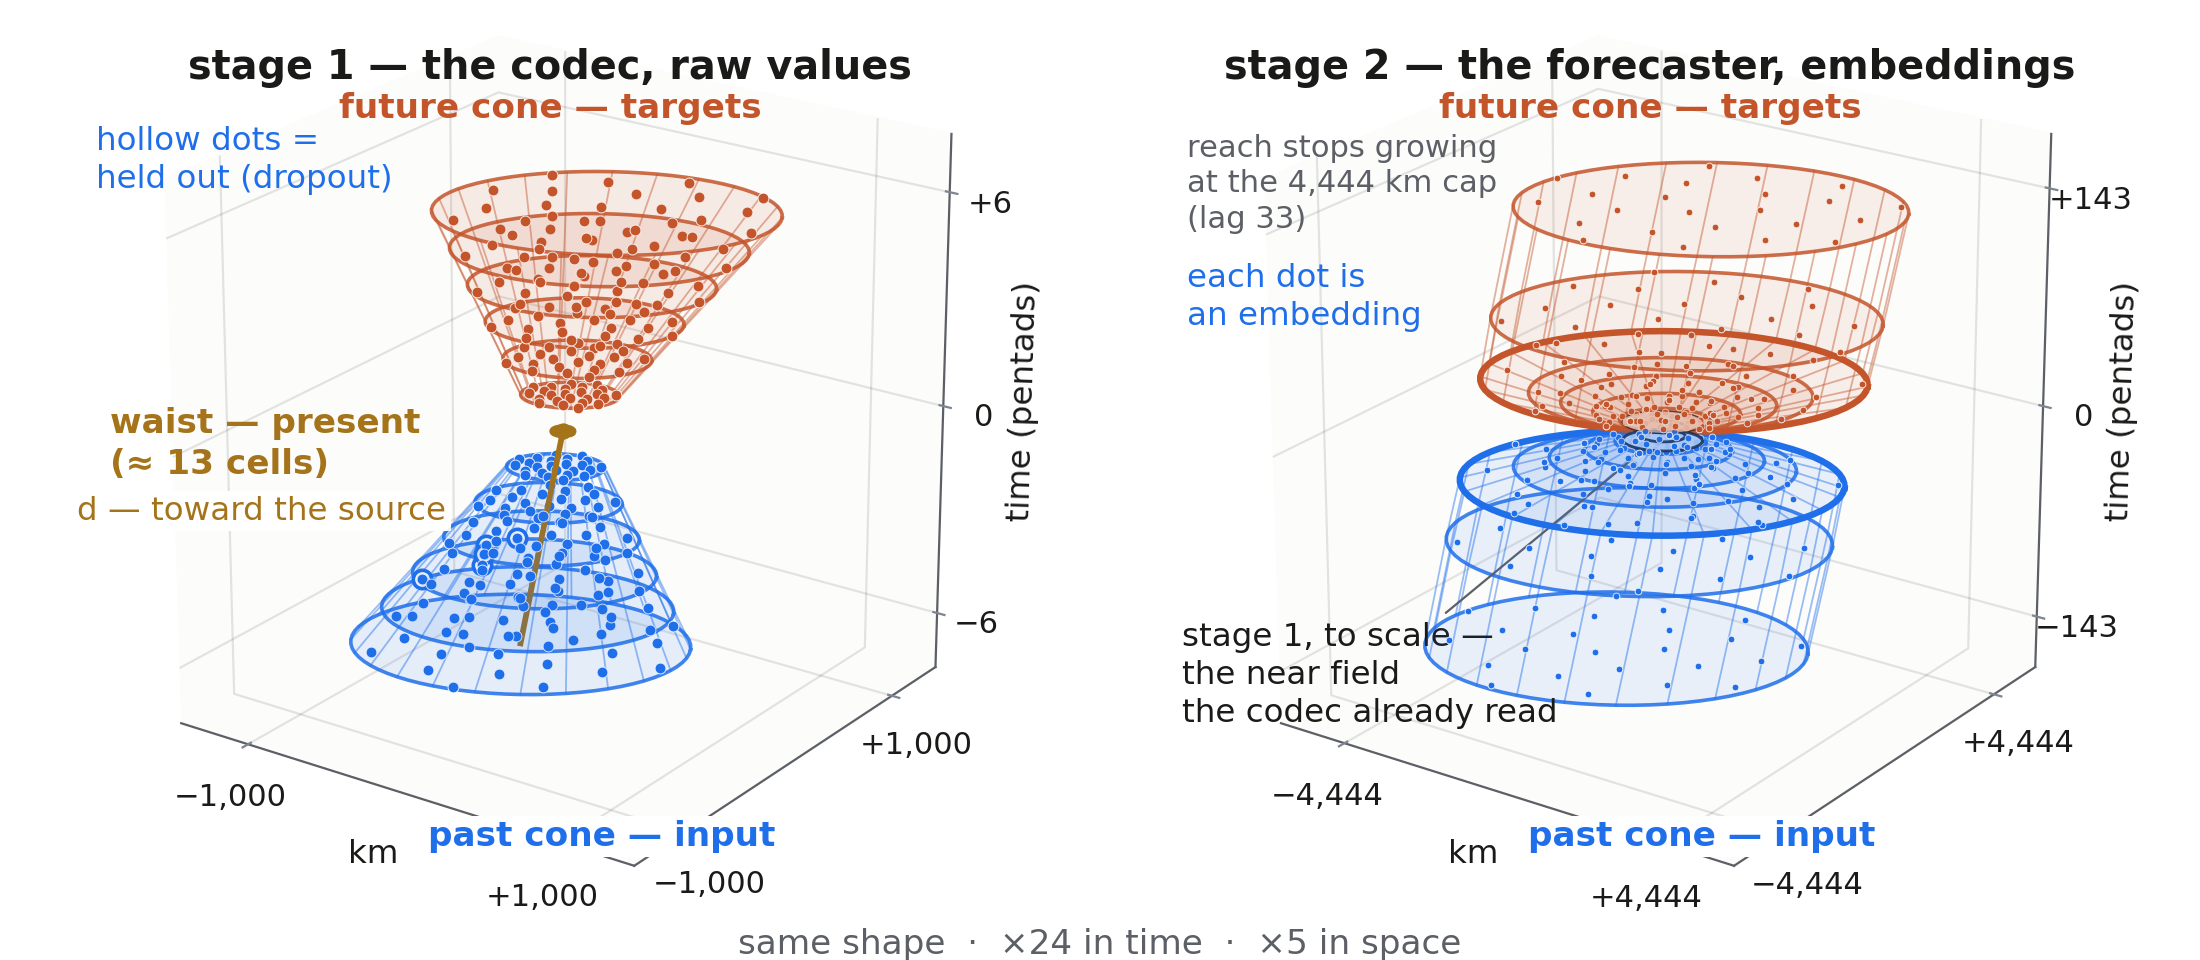
\includegraphics[width=\linewidth]{fig_hourglass.png}
\caption{The hourglass at both scales. Each lag is a footprint of 24
sampling points (a Vogel sunflower, phase-rotated by the golden angle per
lag so consecutive slices interleave) inside an ellipse whose size grows
with lag; the past half is input, the waist is the present, the future half
is target only. Left: stage~1 over raw values, six pentads each way,
${\approx}$900\,km at six pentads for the ocean-surface channels, a waist of
thirteen cells. Right: stage~2 over stage-1 embeddings, 7--143 pentads each
way, opening to a 4{,}444\,km cap; stage~1's whole hourglass is the small
solid at the centre.\label{fig:hourglass}}
\end{figure}

\section{The data as the model sees it}\label{sec:data}

Nothing is resampled to a common grid at storage time. Every source is stored
at its own resolution and cadence in one of three tiers, the sampler turns
all of them into one token at read time, and the decoder is queried at a
location \emph{and} a footprint. The programme's families of data are the
instances of these tiers; this section describes them as the model sees them.

\subsection{The global tensor}\label{sec:data-tensor}

\paragraph{Grid and time axis.} The dense backbone is a global tensor on a
point-aligned $0.25^\circ$ grid --- latitudes $-90 + 0.25\,i$, $i =
0,\dots,720$, longitudes $-180 + 0.25\,j$, $j = 0,\dots,1439$, so $721\times
1{,}440 = 1{,}038{,}240$ cells, rows south first, longitude wrapping at the
dateline --- at a fixed five-day bin, the \emph{pentad}, counted from
1982-01-01: bin $b$ covers days $[5b, 5b+5)$, and the record 1982-01 to
2024-12 holds 3{,}142 bins. A bin is an averaging window, not a date; a year
holds 73 of them and none aligns with a month. A coarse $1^\circ$ grid of
$181\times360$ points is defined the same way, and a coarse channel is read
at a fine position by nearest coarse point, so the sixteen fine cells under
one coarse cell see one number. That is the model's honest view of a coarse
product and it is not interpolated.

\paragraph{Channel groups.} Channels are stored in groups, each at its own
native grid and cadence, each an array $[T, H, W, C]$ in float16, bin-major
so that one time step of one group is one contiguous byte range:
\begin{itemize}
\item \textbf{ocean surface} at $0.25^\circ$, every pentad: surface current
speed and its two components, sea-surface height and log mixed-layer depth
from the GLORYS reanalysis (1993--), sea-surface temperature and sea-ice
concentration from OISST (1982--) --- seven channels, defined over ocean
cells;
\item \textbf{atmosphere and land} at $1^\circ$, every pentad, over every
surface: wind stress and its within-pentad standard deviation (four
channels), 2\,m air temperature, 10\,m wind (two), surface pressure,
precipitation rate, snow water equivalent, soil moisture and temperature in
the top 10\,cm, the latent and sensible heat fluxes, and the skin
temperature --- fifteen channels from the NCEP reanalysis, with ERA5 at the same
grid as the intended replacement;
\item \textbf{ocean interior} at $1^\circ$ and monthly cadence: temperature
and salinity at sixteen pressure levels from 10 to 1{,}900\,dbar from the
Roemmich--Gilson Argo climatology (2004--), 32 channels, each month written
into the pentad that contains its fifteenth day;
\item \textbf{ocean colour} at $0.25^\circ$ from September 1997: the block
mean of $\log_{10}$ chlorophyll over the $6\times6$ OC-CCI 4\,km cells under
each point and the fraction of cell-days in the block that were observed
--- the second channel says how much evidence the first rests on;
\item \textbf{statics}: a surface class per cell (702{,}642 ocean, 226{,}495
land, 107{,}074 ice sheet or glacier, 2{,}029 inland water; ice takes
precedence over ocean on an ice shelf because that is the surface an
instrument sees) and elevation.
\end{itemize}
No channel is masked by sphere. A land cell reads its skin and air
temperature and its soil state, an ocean cell its surface fields, and every
cell reads the shared atmosphere; the observed sea-surface and land-surface
temperatures are separate channels because they measure different things
with different instruments. A channel is a quantity and an instrument, never
a sphere.

\paragraph{Standardisation, transforms and missing values.} Every stored
value is standardised, $x' = (x - \mu)/\sigma$, with $(\mu, \sigma)$ over all
finite values of the channel. Anomalies are not stored: at load time every
channel enters as a standardised anomaly against a day-of-year harmonic
climatology (annual and semi-annual terms) fitted on training years only and
divided by a training-year standard deviation, so nothing in the
climatology, the scale or the normalisation of any read-out sees a held-out
year. Log-normal quantities (mixed-layer depth, chlorophyll, precipitation,
snow water equivalent) are transformed before standardisation; bounded
fractions (sea-ice concentration, soil moisture) through a logit. A value
that does not exist at a cell and bin --- a land cell's sea-surface
temperature, a month without an Argo field, a colour cell under cloud ---
is not a zero: every token carries an \emph{observed} flag per channel, an
unobserved entry is masked from the loss and from the encoder's input, and
the tensor's own holes are the sources' holes, counted per channel and bin
at build time.

\subsection{The fine-granularity families}\label{sec:data-fine}

The $0.25^\circ$ pentad tensor is the coarsest thing the model reads. Three
facts decide how finer sources enter. A coarse value copied into fine cells is
a lie the model cannot see through: nine copies of one reanalysis value are
not nine measurements. A fine value averaged into a coarse cell throws away
exactly what the finer source was bought for: a 4\,km colour field averaged
into $0.25^\circ$ keeps one part in thirty-six. And \emph{missing} is not
damage and neither is \emph{far away}: the nearest profile to a cell is
information whose value depends on its distance, and a grid cell hides that
distance. So finer sources are stored by their density --- what a read costs
--- rather than by their sphere or their science, in three tiers with one
registry:

\begin{itemize}
\item \textbf{Tier G, gridded dense}: fields at or finer than about 4\,km,
daily to monthly, near-complete coverage --- ocean colour at 4\,km (OC-CCI,
1997--), level-3 sea-surface temperature at 5.6\,km per sensor (SST CCI) and
2.2\,km merged (ACSPO), sea ice at 6.25\,km on polar grids, 4\,km
geostationary cloud-top temperature, 0.1$^\circ$ daily precipitation
(IMERG), and on land the daily $0.05^\circ$ land-surface temperature, snow
and surface reflectance fields. A group finer than $0.25^\circ$ is stored
\emph{sharded}: one compressed file per group and pentad, holding one frame
per day (or per three hours), cut into $256\times256$-pixel tiles with a
byte index per tile, so a read fetches only the tiles around the anchor and
an empty tile costs nothing. The footprint is a constant per group.
\item \textbf{Tier P, points, profiles and tracks}: everything sparse in
space or time --- Argo and BGC-Argo profiles, every non-Argo ocean profile
since 1772 (WOD), ship and buoy reports since 1662 (ICOADS), ship bottle
chemistry (GLODAP), surface drifters, the tropical moored arrays, open-ocean
moorings, the Atlantic overturning arrays' own instruments, surface CO$_2$
(SOCAT), along-track altimetry at 7\,km and SWOT swath samples at 2\,km,
column CO$_2$ soundings, wave height along track; on land, weather stations
and balloon soundings, tide gauges, coastal buoys, gliders, flux towers,
active-fire detections, river discharge, soil probes, orbital LiDAR
footprints. A store is a set of column arrays --- time in integer seconds,
latitude, longitude, values, observed mask, quality, a hashed platform
identity, a per-row footprint --- sorted by pentad bin with an index of where
each bin starts, so the $k$ nearest observations to an anchor within a
space--time radius are one bounded scan. Observations before 1982 keep
negative bins; the reader clips to the axis in use.
\item \textbf{Tier T, tiles}: fine imagery at or under a kilometre ---
Sentinel-1 and -2, Landsat, NISAR, OLCI and SLSTR, VIIRS, MODIS at 1\,km ---
is \emph{not} stored as values. The store is a catalogue of scene-dates
(footprint polygon, sensor, time, cloud and valid fraction, location) and a
\emph{token cache}: a small local codec (\S\ref{sec:data-tile}) encodes one
tile-date into a few 64-dimensional vectors, which are stored as a tier-P
store whose ``values'' are those vectors, with footprint equal to the tile
and the day. Google's published AlphaEarth embedding \cite{alphaearth} ---
64 numbers per 10\,m of land per year --- enters through the same path as a
ready-made token cache, which is what allows the programme's own tile codec
to be measured against it with everything else held fixed.
\end{itemize}

The global fine-granularity family --- the ocean and the air measured at
10\,km or finer and every five days or finer --- is the concrete instance
of tiers G and P above the $0.25^\circ$ tensor (Table~\ref{tab:gf}); its
land-and-coast counterpart holds the station networks, gauges, towers, fire
detections, rivers, the daily $0.05^\circ$ land fields, the imagery
catalogue and the land-change targets, and a third family is that
counterpart with the imagery catalogue replaced by the AlphaEarth embedding.
Two rules govern admission to the family. Raw measurements first: a derived
product is admitted only where it carries measurements nothing else does,
and gap-filled analyses are not admitted; three sources slightly coarser
than the rule --- scatterometer wind at 12.5\,km, satellite rainfall at
11\,km, one column-CO$_2$ sounder at 10.5\,km --- are named exceptions. And
every store must lower the model's error on one of the four read-outs, on
the comparison of \S\ref{sec:eval-compare}, or be dropped. Sources already
held elsewhere --- the reanalysis and level-4 fields of the tensor, the Argo
profiles, the drifters, tropical moorings, ship CO$_2$ and along-track sea
level of the point families --- are not rebuilt.

\begin{table}[t]
\centering\scriptsize\setlength{\tabcolsep}{3pt}
\begin{tabular}{@{}L{1.6cm}L{4.1cm}L{2.2cm}L{1.9cm}L{1.9cm}L{2.0cm}c@{}}
\toprule
store & what it is & producer & space & time & record & tier \\
\midrule
\code{seaice\_asi} & daily sea-ice concentration from microwave radiometers & Univ.\ Bremen, AMSR-E/2 & 6.25\,km polar grids & daily & 2002--11, 2012-- & G \\
\code{oc4k} & daily ocean colour: chlorophyll, attenuation, reflectance & ESA OC-CCI v6.0 & 4.6\,km & daily & 1997-09-- & G \\
\code{sst\_cci05} & daily sea-surface temperature per sensor & ESA SST CCI v3.0 & 5.6\,km & daily, day and night & 1979-07-- & G \\
\code{sst\_acspo02} & daily sea-surface temperature merged across sensors & NOAA ACSPO & 2.2\,km & daily, AM and PM & 2000-02-- & G \\
\code{irtb} & cloud-top brightness temperature from geostationary satellites & NOAA CPC & 4\,km & 30\,min (3-hourly first) & 1998-01-- & G \\
\code{precip01} & daily satellite precipitation (IMERG) & NASA/JAXA GPM & 11\,km & daily & 2000-- & G \\
\code{wind12} & ocean wind from scatterometers & EUMETSAT OSI SAF; QuikSCAT & 12.5\,km swath cells & per pass & 1999--2009, 2007-- & G \\
\code{swot} & sea-surface height across two 50\,km radar swaths & NASA/CNES SWOT & 2\,km & per pass, 20.86-day cycle & 2023-07-- & P \\
\code{swh} & significant wave height along altimeter tracks & ESA CCI Sea State & ${\approx}$7\,km along track & 1\,Hz & 1991-08--2023-12 & P \\
\code{icoads} & ship and buoy weather reports & NOAA NCEI / NCAR, ICOADS 3.0 & point & per report & 1662-- & P \\
\code{wod} & ocean temperature, salinity and oxygen profiles, Argo excluded & NOAA NCEI, WOD & point profile & per cast & 1772-- & P \\
\code{glodap} & ship bottle samples of carbon, nutrients and oxygen at depth & GLODAPv3 & point bottle & per cruise & 1972--2023 & P \\
\code{bgcargo} & floats measuring oxygen, nitrate, pH, chlorophyll, backscatter & Argo GDAC, BGC-Argo & point profile & ${\approx}$10 days per float & 2002-- & P \\
\code{oceansites} & fixed open-ocean moorings & OceanSITES & point mooring & hourly or finer & 1980s-- & P \\
\code{deep\_arrays} & the instrument records of the four Atlantic overturning arrays & RAPID/MOCHA, OSNAP, SAMBA, MOVE & point mooring & 15\,min--1\,h & 2000 / 2004 / 2009 / 2014-- & P \\
\code{xco2} & column-averaged CO$_2$ soundings & NASA OCO-2, OCO-3; GOSAT & $<3$\,km$^2$ sounding & per sounding & 2014-06-- & P \\
\bottomrule
\end{tabular}
\caption{The global fine-granularity family: the ocean and the air at 10\,km
or finer and five days or finer, as the model reads it. Each store is
stored at its own resolution and cadence in its tier and enters through the
token schema of \S\ref{sec:data-token} with its own footprint. Sizes range
from tens of megabytes (the bottle samples) to a few terabytes (the
kilometre-scale temperature fields); a one-month test fetch through the real
builder replaces every estimate before a store is built.\label{tab:gf}}
\end{table}

Three properties make the tiers one family. One time axis: every tier is
indexed by the pentad bin from the 1982 epoch, tier-P rows keeping their
exact time inside the bin so $\Delta t$ is fractional. One registry: a JSON
file per family lists every group with its tier, layout, cadence, channels
and units, footprint constants, first bin, file checksums, sources, licence
and builder commit, and a consumer dispatches on the tier, so a new group is
an entry and not a code path. One sampler contract: \code{gather(anchor,
family)} returns, for each group, tokens in the schema of
\S\ref{sec:data-token} under that group's cone family, with a fixed slot
count per group so that batches stay rectangular. Datasets whose licences
forbid redistribution are stored on a private track in the same format,
listed in the public registry, and never republished; a model trained on
them is published only where the licence's terms on derived works allow it.

\subsection{The local codec for tiles}\label{sec:data-tile}

A $64\times64$-pixel tile at 10\,m is 4{,}096 pixels of 13 bands, and a
$0.25^\circ$ cell holds some seven thousand of them; they cannot be sampling
points. The local codec is a masked autoencoder over one tile-date --- all
bands, the sensor's own metadata (resolution, incidence angle for radar, sun
angle for optical) as conditioning, so that one codec with a learned
\emph{source} embedding serves optical and radar sensors alike --- whose
objective is masked-pixel reconstruction plus a same-place-different-date
contrastive term, so that the token carries state rather than texture. It
outputs $k = 4$--$8$ tokens of 64 dimensions per tile-date, cached once and
reused by every anchor whose cone contains the tile. It has snapshot
semantics by construction: it sees one date, and the cone codec supplies the
time axis by reading the cached tokens of many dates. The tile size is a
knob to be measured, not a constant: at 640\,m tiles and seventy clear dates
a year the global token cache is of order 20\,TB per year; at 2.56\,km it is
sixteen times smaller and still a hundred times finer in area than a
$0.25^\circ$ cell. Raw imagery is streamed once to train and once to encode,
and never kept.

\subsection{One token schema}\label{sec:data-token}

The unit the encoder attends over is a place at a time, carrying every
channel present there:
\begin{equation}
\text{token} = \big(\,\mathbf{v}[C],\ \mathbf{m}[C],\ \Delta x,\ \Delta y,\
\Delta z,\ \Delta t,\ \log_2 f_p,\ \log_2 f_t,\ n_R,\ s,\ \text{sphere},\
\text{season}\,\big),
\end{equation}
where $\mathbf{v}$ is the vector of standardised anomalies of the group's
channels and $\mathbf{m}$ the observed flag per channel; $(\Delta x, \Delta y,
\Delta z, \Delta t)$ is the offset from the anchor in kilometres, metres of
depth or height, and days; $\log_2 f_p = \log_2(\text{footprint
km}/27.83)$ and $\log_2 f_t = \log_2(\text{support days}/5)$ are the
spatial and temporal support of the measurement in units of a $0.25^\circ$
cell and a pentad, clamped to $\pm12$ (a Sentinel-2 pixel reads $(-11.4,
-4)$, an Argo profile $(-4, -4)$, a 4\,km daily colour cell $(-2.8, -2.3)$,
an OISST pentad cell $(0, 0)$, a reanalysis cell at its true spectral
support $(+2.9, 0)$, a monthly $1^\circ$ Argo field $(+2, +2.6)$); $n_R$ is
how many observations of this kind were within reach; $s$ is a learned
source embedding (sensor or product class); and the sphere code and the
day-of-year harmonics of the token's own time complete it. One token per
sampled location and lag, \emph{not} one per channel per location: the
channel dimension lives inside the token, so the token count is the
geometry's and not the channel count's, and adding a channel costs a vector
entry rather than a token. The two footprint fields are constants per group
for dense sources and per row for sparse ones, and nothing else in the schema
depends on the tier: the encoder never learns which file a value was read
from, only what it is, where and when it is, and how much it averaged.

Offsets are what correct the coarse-value problem. A $1^\circ$ cell's value
is one token located at the cell centre, seen from sixteen different
$(\Delta x, \Delta y)$ by the sixteen anchors inside it, and the present-day
patch of a fine anchor holds one such token, not nine copies. Point
observations enter as tokens of the same schema placed where and when they
were observed --- the $k$ nearest profiles, drifters or stations in
space--time within the cone, $k$ small (three to eight per depth group),
one-sided in time, padded to a fixed $k$ with \emph{miss} tokens --- and
there is no ellipse to learn for them, only the attention over what was
measured. A token whose value the encoder is not allowed to see carries a
\emph{hidden} marker, distinct from the \emph{never observed} marker: a
value we hid and a value the data never had are different facts.

\subsection{The holdout}\label{sec:data-holdout}

Three development years --- 2009, 2017 and 2023 --- are held out of
training, of the climatology and of every statistic, for model selection;
the terminal test is one scoring of a model trained on data up to 2020 on
2021--2024, run once. A training example is admissible only if every bin
its forward pass can see --- every past-cone token, every future-cone target
--- is a training bin, and that admissibility is certified by brute force
over a large draw of anchors before a run starts; a non-zero count refuses
the run. Longitude holes are held out in addition, so that extrapolation
into an unseen region is scored separately from interpolation inside a seen
one.

\section{The hourglass and its learnable geometry}\label{sec:geometry}

\subsection{Waist, past cone, prediction cone}\label{sec:geometry-shape}

\paragraph{The waist.} The present is a disc of radius two cells at
$0.25^\circ$ --- about thirteen cells, sampled as a small sunflower so that
every bearing is represented --- read as input and reconstructed, and the
embedding $z$ is written for the anchor at its centre. The waist exists
because the quantities the read-outs depend on are gradients: thermal wind
is a horizontal density gradient, geostrophic velocity a slope in sea-surface
height, and a gradient does not exist inside one cell. The waist carries the
same shape parameters as the cone evaluated at lag zero, so a boundary
current can have a waist elongated along the flow.

\paragraph{The past cone.} Lags $1$--$6$ pentads, every pentad, so that the
codec owns the last thirty days at full cadence: five days is the finest
cadence the dense tensor has, and the thirty-day window is the codec's whole
job. At each lag and for each channel group the dense sampling set is a
24-point sunflower --- the Vogel spiral at the golden angle --- mapped
through an ellipse. The footprint at lag $\ell$ is Gaussian with centre
$\ell\,\mathbf{d}$ from the anchor and covariance
\begin{equation}
\Sigma(\ell) = \Sigma_0 + \ell^2\,\Sigma_v,
\qquad p(\ell, i) = \mathbf{x}_{\text{anchor}} + \ell\,\mathbf{d} +
\Sigma(\ell)^{1/2}\,\mathbf{u}_i ,
\end{equation}
where $\mathbf{u}_i$ are the canonical sunflower points on the unit disc,
$\mathbf{d}$ is the drift per pentad --- the arrow toward the source ---
$\Sigma_0$ is the waist ellipse and $\Sigma_v$ the velocity-spread ellipse,
so that the footprint's standard deviation grows linearly with lag, which is
the reach-grows-with-lag rule of the cone argument. Time is not
sunflower-sampled --- one slice per pentad --- but a stack of identical
slices repeats the same bearings at every lag, so the sunflower's phase
advances by the golden angle from one lag to the next
($\text{bearing}_{i,\ell} = (i + \ell)\times137.5^\circ$) and the six slices
interleave in space--time at no cost. The anchor's own column is always
sampled at every lag.

\paragraph{The far ring.} In addition to the ellipse, every lag keeps one
fixed ring of 24 points at log-spaced radii from 28\,km out to the lag's
design reach $v_{\text{design}}\,\Delta t\,(1 + \ell)$, capped at the
antipode, read at full weight and never gated. The design speed is the maximum measured speed of the fastest mechanism that carries
the family's information, times a safety factor of $1.5$ (for the ocean,
the Somali Current and the first-baroclinic Kelvin wave at 3.6\,m\,s$^{-1}$,
so $5.4$\,m\,s$^{-1}$ and 2{,}333\,km per pentad; for wind stress the
atmosphere, which is global within one pentad). The factor covers three
things at once: a pentad mean on a $0.25^\circ$ grid under-reads peaks, the
maxima are literature values rather than the true extreme, and a warming
ocean may run faster. The ellipse gives the cone direction and density; the
ring guarantees that no driver is excluded by construction. A cone that is
too wide costs tokens, a cone that is too narrow excludes true causes
silently, and the buffer is spent on the cheap side.

\paragraph{The prediction cone.} The past cone point-mirrored through the
anchor: centre $-\ell\,\mathbf{d}$, the same $\Sigma(\ell)$, leads $+1$ to
$+6$ pentads, sampled the same way and read by nobody. Each point in it is a
decoder query and a target only. The anchor column at every lead is always
among the targets, which is what makes the fixed-frame forecast that stage~2
consumes always trained.

\subsection{Channel families and the per-channel aperture}\label{sec:geometry-aperture}

\paragraph{One direction per flow, one scale and one memory per channel.}
What is shared per region, lag and channel group is the shape $\Sigma(\ell)$
and the drift $\mathbf{d}$: everything the water carries is carried the same
way, so the arrow toward the source and the elongation along the jet are
properties of the flow and not of the tracer. What is per channel is a
log-scale $s_c$ (two for the L-shaped channels, lags $0$--$1$ and $2$--$6$)
and a memory $\tau_c$: in space $\Sigma_c(\ell) = e^{s_c}\,\Sigma(\ell)$ ---
the same ellipse inflated or shrunk, never turned --- and in time lag $\ell$
is weighted by $e^{-\ell\Delta t/\tau_c}$, how far back the channel is worth
reading. Both are initialised from a table of families set by physics: wind
stress at 500\,km within a ten-day memory (so lags $0$--$1$ count and lag 6
is at $e^{-3}$); currents, sea-surface height and the profile tokens at
130\,km per pentad with a long memory; sea-surface temperature and
mixed-layer depth at $\max(\text{that}, 500\,\text{km})$ at lags $\le 1$,
where the atmosphere stirs them, and the ocean's growth thereafter; land at
400\,km flat and a long memory, because soil does not advect; the depth
column with no ellipse of its own. At step zero every channel reads exactly
the reach and the lags the table gives it.

\paragraph{The aperture, at zero extra tokens.} Because a token carries all
channels of its group, each channel reads the group's shared points through
its own weight,
\begin{equation}
w_{c,i,\ell} = \exp\!\big(-\tfrac12\,p_i^{\top}\Sigma_c(\ell)^{-1}p_i\big)\,
\exp\!\big(-\ell\,\Delta t/\tau_c\big),
\end{equation}
applied to that channel's value and observed-flag entries before the token's
projection. A point outside channel $c$'s aperture in space or beyond its
memory in time contributes about zero for $c$ and still carries the other
channels at full weight; a point 400\,km from the anchor at lag~1 is read by
the currents at about 30\% and by sea-surface temperature at about 73\% at
the initial apertures, from one token and one read. The aperture is a smooth
function of $\Sigma_0$, $\Sigma_v$, $\mathbf{d}$, $s_c$ and $\tau_c$, so the
loss reaches all of them through every candidate point at once --- a far
better gradient than the four neighbouring cells an interpolated read would
give, and the reason the geometry can learn without the data loader knowing
where it currently is. The far ring is not gated: a safety net the model can
switch off is not one.

\subsection{The learnable parameters and their guards}\label{sec:geometry-learn}

\paragraph{Eight dimensionless numbers per $1^\circ$ cell and channel
group.} The drift is stored as $\mathbf{d} = \tanh(\mathbf{x})\,
v_{\text{design}}\Delta t$, capped at the design speed by construction. The
two ellipses are stored as matrix logarithms,
\begin{equation}
S = \log\Sigma = m\,\mathbf{I} + k\begin{pmatrix}\cos2\theta & \sin2\theta\\
\sin2\theta & -\cos2\theta\end{pmatrix},
\qquad m = \ln\sigma_1 + \ln\sigma_2,\quad k = \ln\sigma_1 - \ln\sigma_2 ,
\end{equation}
whose trace is the size and whose traceless part is the log aspect ratio
times the double-angle phasor: no parameter is in kilometres, no angle
wraps at $180^\circ$, a circle is the natural zero, and --- the reason for
the form --- an Adam step of one learning rate moves every radius by the
same fraction of itself whatever its size \cite{adam}, where a radius stored
in kilometres would be frozen at a thousand kilometres and twitchy at
thirty. The waist's eigenvalues are floored at one cell (28\,km) and
$\Sigma_v$'s at the design speed by a softplus offset in log space rather
than a clip, so the floor never kills the gradient. The per-channel $s_c$ and
$\tau_c$ are global, about a hundred numbers in all.

\paragraph{Where they live.} On a $1^\circ$ map per channel group
(64{,}800 cells; ocean maps live over ocean, land maps over land), the
anchor's parameters being the bilinear blend of the four surrounding cells,
so the geometry varies smoothly and never jumps at a cell edge. One degree
because the currents that carry the overturning are about 100\,km wide ---
the Florida Current runs through an 80\,km strait --- and a $10^\circ$ cell
would average the Gulf Stream with its recirculation and learn a drift near
zero. Against noise in data-poor cells, each map is a coarse $10^\circ$ map
plus a $1^\circ$ residual under an L2 shrinkage and a Laplacian smoothness
prior with one weight, so a cell at the ice edge or along a coast inherits
its region's arrow rather than fitting noise; each $1^\circ$ cell still sees
sixteen anchors over three thousand pentads for its eight numbers. There is
one map per channel group --- ocean surface; atmosphere, with drift only
inside its memory; land, with no drift --- and none for the depth column,
whose tokens are the nearest profiles with their own offsets and depths. All
told about $1.6$\,M nominal parameters, half of them live, and no compute. A
first-harmonic seasonal term on the drift, $\mathbf{d}(\tau) = \mathbf{d}_0
+ \mathbf{d}_1\cos\tau + \mathbf{d}_2\sin\tau$, is a second-phase option for
monsoon regimes where the current reverses.

\paragraph{How they learn: gate first, harden later.} In the first phase the
candidate points per region and group are fixed --- a log-radial set of 36
per lag out to the design reach, plus the anchor column --- so that the
loader's reads are regular, cacheable and never depend on live weights, and
the geometry learns only through the aperture weights over those candidates.
Every $N$ steps (2{,}000 to start) the dense sunflower table per region is
re-baked from the current ellipses and the loader swaps tables at an epoch
boundary; within an epoch reads stay regular. The geometry parameters get a
learning-rate multiplier of ten over the codec's, the practice of deformable
attention \cite{deformable}, recorded per run. Reading at continuous
positions through a deformable gather was considered and rejected: it
couples the loader's read pattern to the live weights, and its gradient sees
only the four cells around each point.

\paragraph{Why a learnable cone can cheat, and the guards.} If target
positions could move, the gradient would move them to smooth open water,
away from fronts --- a lower loss that means nothing. Five rules close the
ways of doing so. The loss reaches the geometry only through the
\emph{input} reads; target positions carry a stop-gradient and are treated as
constants. The future cone is tied to the past cone by the mirror, so it
cannot be tuned on its own; an untied arm is an ablation, not the design.
The evaluation geometry is frozen to the fixed hourglass for every arm, so
two runs with different learned cones are scored on the same questions. The
aperture never enters the loss weights: in the gate phase the targets are the
fixed mirrored candidate set with fixed weights, so a model that narrows its
aperture gains nothing on what it is scored on. And the far ring is kept and
never gated. A residual second-order effect remains --- as the input cone
moves, the mirrored targets move with it --- and is monitored rather than
assumed away: every evaluation reports the variance of the targets under the
learned cone against the fixed cone, and a drop of more than 10\% is a flag
that the geometry is drifting toward easy water rather than toward the
source.

\paragraph{Initialisation.} $\mathbf{d} = 0$; $S_0$ the log of an ellipse
of the waist's radius with the measured flow anisotropy of $0.71$; $\Sigma_v$ from the
family table's speed; $s_c$ and $\tau_c$ from the same table --- the fixed
hourglass exactly, so that step zero of the learned arm \emph{is} the
control and every departure from it is something the data asked for.

\section{Stage 1: the codec}\label{sec:stage1}

\paragraph{Tasks.} Each training example is one anchor at one bin and draws
one of four tasks (Table~\ref{tab:tasks}). Dropout patterns for the nowcast
and the fill-in fire independently, each with its own probability: one
channel hidden at the waist only; the most recent lags hidden (every point at
lag $\le \ell_0$, $\ell_0 \in \{1, 2, 3\}$), so the model must extrapolate
from stale history; a $90^\circ$ bearing wedge hidden, so it cannot lean on
one direction; points hidden at random ($p = 0.3$), imitating sparse
observation; and, for the nowcast only, the whole waist. The task is not
told to the model by a token: the hidden and never-observed markers are
visible and the lead is in every query's coordinates, which is enough.
Within an example the loss weights are equal across tasks; the shares set
the mix and are recorded per run.

\begin{table}[t]
\centering\footnotesize
\begin{tabular}{@{}L{2.5cm}L{3.5cm}L{2.7cm}cL{3.6cm}@{}}
\toprule
task & input & targets & share & what it teaches \\
\midrule
T1 forecast & waist + past cone & future cone & 0.35 & the full problem \\
T2 snapshot forecast & waist only, past cone hidden & future cone & 0.15 & the built-in twin: what history buys, inside one model \\
T3 nowcast from history & past cone under a dropout pattern; waist hidden & waist & 0.25 & the present from the past: persistence, advection, memory \\
T4 fill-in & waist + past cone, both under a dropout pattern & the hidden waist cells and points & 0.25 & reconstruction from partial observation \\
\bottomrule
\end{tabular}
\caption{The four tasks of stage~1, drawn at random per example. Shares are
a starting point and the first thing the comparisons of
\S\ref{sec:eval} vary.\label{tab:tasks}}
\end{table}

Three rules are not knobs. \emph{Knowable targets only}: a target's channel
must be visible somewhere in the input, at some lag, or the target is
unknowable and teaches the model to predict the mean; the sampler enforces
this and logs the count of violations, which is required to be zero.
\emph{No copy targets}: the waist family scores hidden channels only,
because a target the model can read off the input is not a question.
\emph{Every family against its own bar}: the loss per task, family and lead
is reported against the score of predicting the mean, and a family is
called learned only where the ratio is below one at held-out anchors.

\paragraph{Model.} A masked autoencoder in the strict sense \cite{mae}: the
encoder sees only visible tokens and visible channel entries, never a
placeholder for a hidden one. The encoder is a transformer over the
${\approx}300$ per-location tokens of one example --- Perceiver-style
cross-attention into a fixed latent set \cite{perceiver} where a fixed-size
interface is wanted, a plain encoder with a learned attention pool otherwise
--- producing $z$ of width 128--256. The bottleneck is in the token count,
not in the width: what the forecaster needs compressed is the near field's
thousands of values into one vector per cell, and a narrow $z$ is where
capacity fights between the waist and the cone. The decoder is query-based
and reads $z$ alone: a query is (offset, channel, sphere, depth or height,
lead, footprint), it cross-attends to $z$, and its head emits a mean and a
log-variance per channel group. A decoder that could also read the encoder's
latents would let $z$ carry nothing; that path is closed. At the ladder's
larger rungs (\S\ref{sec:scale}) the feed-forward block becomes a mixture of
experts routed by sphere code and channel group, because the value vectors
differ by sphere in statistics and physics and expert specialisation is the
natural fit at constant active parameters.

\paragraph{Objective.} A heteroscedastic Gaussian likelihood per channel
group in its transformed space, in the decoupled form
\begin{equation}
\mathcal{L} = \|\mu - y\|^2 \;+\; \tfrac12\, e^{-s}\,(y - \mathrm{sg}[\mu])^2
+ \tfrac12\, s, \qquad s = \log\sigma^2 ,
\end{equation}
so that the mean is trained by plain squared error --- what the forecaster
consumes and what every score measures --- while the variance is trained by
the likelihood with the mean detached. This removes the known pathology of
heteroscedastic regression in which the variance head explains a hard target
away instead of the mean learning it \cite{betanll}; the $\beta$-weighted
likelihood of that paper at $\beta = 1$ has the same gradient on the mean.
$s$ is clamped to $[-8, 8]$, the first 2{,}000 steps run at fixed $\sigma =
1$, and the likelihood is per channel group: Gaussian on standardised
anomalies for the continuous fields, Gaussian in log space for the
log-normal ones, a hurdle model (Bernoulli wet or dry times a log-Gaussian
amount) for precipitation, and a logit-Gaussian for bounded fractions.
Every family --- waist reconstruction,
fill-in, each future lead --- is scored at every evaluation against its own
predict-the-mean bar; coverage of the $\pm1\sigma$ and $\pm2\sigma$ bands on
held-out targets is reported as the calibration check.

\paragraph{Weighting across targets.} The squared-error term sums over
targets whose residual errors differ by orders of magnitude --- a persistent
sea-surface temperature at lead one against a wind-stress standard deviation
at lead six --- and a plain sum lets the hardest targets dominate the
gradient. Standardising the targets, which the anomaly transform already
does, weights each by its marginal variance, and that is the wrong scale in
principle: marginal variance conflates \emph{varies a lot} with \emph{hard
to predict}. The right scale for a target is its irreducible error, so the
mean's loss is
\begin{equation}
\mathcal{L}_\mu = \sum_{k} w_k\,\mathrm{MSE}_k, \qquad
w_k = 1 / \mathrm{MSE}_k^{\text{ref}}, \qquad \text{no gradient through } w_k,
\end{equation}
where $k$ runs over (channel, task family, lead) --- a waist reconstruction,
a fill-in point at lag four and a future point at lead three of the same
channel have different residuals and are weighted separately. This is the
stop-gradient form of $\sum_k \log\mathrm{MSE}_k$, i.e.\ Gaussian maximum
likelihood with one fixed variance per target class, so every target
contributes its relative improvement independently of its units; it keeps
the residual scale out of the co-adapting $\sigma$ head, which is what the
decoupled form above is for, and it is the rule behind the sentence that
target classes are weighted explicitly and never through $\sigma$ as a side
effect. The reference is the held-out per-class error, never the final
training-set error, under which an overfitted class's weight explodes. At a
tier with no previous run the reference is an exponential moving average of
the held-out per-class error under stop-gradient, started from the marginal
variance (which the standardisation gives at step zero) and annealed to the
residual over the first few thousand steps; at a tier with a previous run
the weights are frozen from that run's held-out errors, and they are a fixed
point: after a run they are recomputed, and a run is repeated once if any
moved by more than a factor of two. For the heavy-tailed classes ---
precipitation, chlorophyll --- the reference uses a robust scale or the
error a Huber loss. Two things are logged per class: the weighted term
$w_k\,\mathrm{MSE}_k$, which sits near one at convergence and drifts when a
weight is off, and the skill $1 - \mathrm{MSE}_k/\mathrm{var}_k$, which is the
readable number; progress is never judged from the aggregate loss. A
downstream use that cares more about one class's absolute error adds an
explicit multiplier on top, kept separate from the statistical
normalisation.

\paragraph{Training stability.} Embedding collapse is invisible to a
reconstruction loss, because a decoder rescales freely, so the effective
rank of $z$ over a fixed held-out batch and a scale-invariant probe
correlation are logged at every evaluation and a run aborts on two
consecutive sub-threshold readings. No quantisation is switched on from a
random initialisation: a lattice on an untrained encoder collapses within
thousands of steps, whereas a lattice added to a finished continuous codec
does not, so a discrete code, where wanted, is a second phase. Inputs are
standardised, so the gradient clip is $1.0$; AdamW with $\beta_2 = 0.95$,
weight decay $0.1$, a 2{,}000-step warm-up and cosine decay to 10\% of peak;
bf16 with fp32 master weights. Training stops at the held-out minimum with
the minimum's step recorded, and no arm runs past four epochs of anchors
\cite{datacon}.

\section{Stage 2: the forecaster}\label{sec:stage2}

\paragraph{Inputs.} Stage-2 tokens are the codec's embeddings: at each
sampled cell and lag, the mean and log-variance of $z$, the offset
$(\Delta x, \Delta y, \Delta t)$, the statics and the day-of-year harmonics of that
bin. The past cone reads lag 0 --- which already summarises the last thirty
days --- and log-spaced lags $1$, $2$, $3$, $5$, $8$, $13$, $21$, $34$, $55$,
$89$ and $144$ pentads, twelve slices instead of 144, each with the anchor column and a
24-point footprint whose reach follows the fastest \emph{slow} signal ---
planetary waves and gyre adjustment at $0.05$--$0.1$\,m\,s$^{-1}$, about
1{,}000\,km at 34 pentads, the 4{,}444\,km cap from about lag 33 on --- and
a far ring to the antipode at every lag, as in stage~1. Dense sampling where
predictability is dense and sparse where it is not is what keeps an example
at about 300 tokens rather than twenty thousand; the dense 144-pentad window
is the ablation. The same eight-number learnable geometry applies at this
scale with its own $1^\circ$ maps and the same guards. 
\paragraph{The linear backbone.} For the anchor column,
\begin{equation}
\hat{z}_{t+\ell} = \mathbf{G}_\ell\, z_t \;+\; f_\theta(\text{cone}, \ell),
\qquad \mathbf{G}_\ell = \mathbf{U}\,\mathrm{diag}\!\big(e^{-\ell/\tau_j}\big)\,
\mathbf{U}^{-1},\ \ \tau_j > 0 ,
\end{equation}
where $\mathbf{G}_\ell$ is a linear propagator in embedding space with
learned time constants --- contractive by construction, so a free run decays
toward climatology rather than drifting --- initialised from a linear
inverse model \cite{penland} fitted to the training-year embeddings, and
$f_\theta$ is the transformer over the cone with a zero-initialised output
projection. At step zero the forecaster \emph{is} the embedding-space linear
inverse model; whatever it becomes has to earn its distance from it on the
held-out field. Damped persistence is the diagonal special case and is
reported as its own null.

\paragraph{Direct multi-lead targets.} The target is the mirrored future
cone: the anchor column and its footprint at leads $1, 2, 3, 5, 8, 13, 21,
34, 55, 73$ pentads (73 pentads is one year), each lead a query $(\Delta x,
\Delta y, \ell)$ to the same decoder head, predicted directly rather than by
chaining one-step predictions. A direct forecast at lead $\ell$ cannot
compound its own errors, its amplitude is set by the data at that lead
rather than by an accumulation, and the log spacing puts the targets where
the correlation is still changing. The anchor column is weighted 1 and the
off-anchor footprint $0.25$ (a choice); the footprint targets are what make
the prediction a field with coherent advection rather than a set of
independent columns. Leads beyond a year are reached by feeding the
predicted anchor embeddings at leads $1$--$73$ back as the recent past and
querying again: the multi-year roll is a second mode of the same model, not
its training objective.

\paragraph{Objective and calibration.} The decoupled Gaussian likelihood on
each target embedding, weighted per lead and footprint position by the
inverse of its held-out residual error under the rule of \S\ref{sec:stage1}
--- started from the predict-the-mean bar, which is the marginal variance
--- so that every lead contributes its relative improvement and the long,
unpredictable leads do not dominate the gradient; plus a decoded-space term through the frozen
codec decoder for the scoreable channels at leads 1, 8 and 34 (squared error
against the standardised anomaly, relative to climatology), because the
embedding metric is not the metric the forecast is scored on; plus, for the
multi-year mode, a two-step pushforward term in which the model is rolled
once with a stop-gradient on the first step and scored on the second, so it
learns to correct its own errors without back-propagating through the roll.
Under a squared-error mean the conditional expectation shrinks toward zero
as correlation falls, so amplitude calibration is a property of the
objective at the held-out minimum and not a post-hoc fit; the identity
$\mathrm{MSSS}_{\text{clim}} = 1 - (1 + a^2 - 2a\,\mathrm{ACC})$ between the
squared-error skill, the anomaly correlation and the amplitude ratio $a$ of a
forecast against a zero-anomaly reference is logged per lead as the check
that it holds, and a per-lead scaling fitted on training-year starts is
reported as a diagnostic only.

\paragraph{Regularisation.} Three things keep the forecaster in the regime
where it learns rather than memorises. The globe gives every regime of the
ocean and atmosphere as training patterns rather than one basin's; the
log-spaced cone reduces the parameters per example by a factor of seventy
against a dense window; and the model's free part is a residual on a linear
backbone that the data pin down with few degrees of freedom. On top of
these: Gaussian noise on the input embeddings at $0.7$ of the persistence
scale, a denoising objective in disguise; random dropout of past-cone
points; weight decay; early stopping at the held-out minimum with the step
recorded; and, because the model is cheap at this token count, a seed
ensemble of three to five whose spread is the first probabilistic forecast
and whose mean is the deterministic one.

\paragraph{Probabilistic extension.} Once the deterministic level exists, a
shared low-dimensional noise vector per forecast conditions the head so that
samples are coherent across cells and leads, scored by the fair continuous
ranked probability score \cite{crps}. Explicit categorical marginals over a
quantised embedding under the same shared noise are the alternative where
the conditional distribution is two-humped, which at six to twenty-four
months an El Ni\~no index plausibly is; both are decided on the dense field,
never on an index.

\section{The queryable read-out: predicting anything}\label{sec:readout}

The decoder of \S\ref{sec:stage1} is the mechanism by which one model
answers every question, and it is worth stating what it can and cannot do.

\paragraph{A prediction is a query.} A query is a tuple in the same
coordinates as an input token: an offset from the anchor in space, depth or
height, and time; a channel; a sphere; a source class; and a footprint
$(\log_2 f_p, \log_2 f_t)$. ``Channel $c$ at point $p$ at lead $\ell$ over
this footprint'' is one query, and the same decoder answers a $0.25^\circ$
cell over a pentad, a 300\,m pixel on a day, a station at an hour and a
float profile at its depths, because it was trained on targets that carried
exactly those coordinates and footprints. The mean chlorophyll of a
$0.25^\circ$ cell over a pentad and the value of a 4\,km cell on a day are
two different queries of one embedding, and the loss for each is scored
against the observation that actually has that support. The footprint on the
output side is what lets one model be trained on coarse targets today and on
fine targets later without a second head.

\paragraph{Anything the record has contained.} The domain of the read-out is
the set of channels that appear somewhere in the training targets, at the
footprints they appeared with. A channel never observed cannot be asked for;
a footprint far outside the range seen is an extrapolation and is reported
as such. Between those limits the decoder interpolates in coordinate space,
and the same query asked at a place the source never covered --- a
sea-surface temperature over land --- returns a mean with a variance that
says so, because the training targets were masked there and the variance
head has never been rewarded for confidence.

\paragraph{Indices and sections.} A quantity that is a functional of many
cells --- an overturning transport, an area-mean index, a warm-water volume
--- is a head on the predicted embeddings of the cells it depends on: an
attention head over the individual cells of a section, trained on
training-year true embeddings and applied to forecasts, never a head on a
spatial mean, because geostrophic transport is the east--west contrast
across a section and a section mean is the statistic in which that contrast
cancels. The read-out is the cheap, replaceable end of the system; none of
the read-outs is used to choose between models.

\paragraph{Observations as their own truth.} Because point observations are
targets in their own coordinates, a store's own record is the verification
of its forecast: a drifter's velocity, a mooring's temperature at 300\,m, a
gauge's sea level, a tower's CO$_2$ flux. Where a store has a licence that
forbids redistribution, the score can still be published; the values cannot.

\section{Training at scale}\label{sec:scale}

\paragraph{The unit of account.} Data is priced in observed values and their
independence, never in bytes. A $0.25^\circ$ cell is correlated with its
neighbours over a few hundred kilometres and, at the surface, over months,
so a basin's $10^9$ values are of order $10^6$--$10^7$ independent ones ---
the regime in which a small model equals a large one. The globe adds new
regimes, independent by construction; the other spheres add new physics;
daily cadence inside a pentad is mostly the same sample five times; the
kilometre tier adds fine-scale variance that is genuinely new. The ladder's
order follows: globe and spheres first, then footprint, cadence last.
Table~\ref{tab:ladder} prices the rungs against a Chinchilla-style anchor of
one parameter per twenty values \cite{chinchilla}, quoted as a ceiling
because of the correlation above.

\begin{table}[t]
\centering\footnotesize
\begin{tabular}{@{}L{5.6cm}rrrL{4.6cm}@{}}
\toprule
rung of data & values & tokens & ceiling & what it takes \\
\midrule
one basin, $0.25^\circ$ pentads, 42 ocean channels & 2.5\,B & 0.04\,B & 0.12\,B & the pilot's tensor \\
global pentads, four groups and statics & 13.8\,B & 0.21\,B & 0.7\,B & built: the tensor of \S\ref{sec:data-tensor} \\
+ the shared atmosphere and land channels of every sphere & 91\,B & 1.4\,B & 4.5\,B & ERA5, radiometers, scatterometers, gravimetry, soil moisture \\
daily cadence, all spheres & 455\,B & 7.0\,B & 23\,B & a 1.3\,TB tensor and a streaming loader \\
kilometre tier, all spheres & $3.5\times10^{5}$\,B & $5.4\times10^{3}$\,B & --- & not a tensor: the token cache of \S\ref{sec:data-tile}; compute-bound for the first time \\
\bottomrule
\end{tabular}
\caption{The data ladder in observed values; tokens at 65 channels per
token; the ceiling at one parameter per twenty values, an upper bound
because values are correlated.\label{tab:ladder}}
\end{table}

\paragraph{The rungs.} Each rung of the model is bought only on the previous
rung's read-out, under the frozen protocol, with the null ladder of
\S\ref{sec:eval} beside it, and a rung whose held-out minimum arrives inside
2{,}000 steps at full data is over-parameterised, so the next rung is not
bought. L1: a 7--125\,M codec on the global pentad tensor with the fixed and
learned geometries --- the comparisons of \S\ref{sec:eval-compare}. L2: a
0.3--1\,B codec and forecaster on the same tensor plus the tier-P stores,
where the width ladder is re-measured, because it is the one measurement
that tells a data-limited rung from a compute-limited one. L3: 1--4.5\,B
with the sphere-routed mixture of experts on all spheres, where the question
is whether land and atmosphere improve the ocean's rolled skill and vice
versa. L4: daily cadence, the first compute-bound rung, where the question is
whether five times the bytes are worth anything on the terminal holdout. L5:
the kilometre tier, only after L4 has a positive answer. Compute is priced at
$6NT$ per epoch; a 1\,B codec over the global pentad tensor is of order
thirty RTX-4090-hours at four epochs, and the encoder's cost is linear in the
token count because the latents cross-attend to the tokens, so the aperture
and the far ring cost one elementwise multiply per token and no new reads.

\paragraph{Sampling and throughput.} An anchor is a cell and a bin drawn
from the admissible set, uniformly over ocean, land and ice in proportion to
a stated mix; the gather of one example --- the sharded tiles, the point
stores' $k$-nearest scan, the dense slabs --- is host-bound, not
accelerator-bound, and is batched by latitude row so that the per-row dot
tables are reused, with candidate reads regular within an epoch by the
gate-then-harden rule. Every artefact a run produces --- the checkpoint, the
metrics, the geometry maps --- is written incrementally and published to
durable storage while the run is alive, so that a job that dies leaves the
next one nothing to recompute; a training run's configuration is a named
recipe, never a hand-assembled set of flags, and a resumed run derives its
architecture from its checkpoint. A number from a single seed is a direction,
never a level: the first result at every new tier, metric, cadence or codec
buys its own replication, and any probe-scored claim needs three seeds.

\section{Evaluation protocol and pre-registered comparisons}\label{sec:eval}

\paragraph{Protocol.} Held-out years 2009, 2017 and 2023 stay held out of
training, of the climatology and of every statistic; a codec and forecaster
trained on data through 2020 are scored once on 2021--2024 as a terminal
test. For each lead: mean-squared skill against climatology, raw persistence
and damped persistence, anomaly correlation and amplitude ratio, per channel
and per scope (trained and held-out longitudes separately), from three
starts per held-out year, with block-bootstrap intervals over (year, start)
\cite{goddard}. The null ladder beside every read-out is climatology,
persistence, damped persistence (a per-cell AR(1) fitted on training years),
the linear inverse model in data space and in the rung's embedding space
\cite{penland,newman}, an analogue (retrieval) forecast, and the previous
rung; a learned model is reported against all of them. A configuration is
compared to another on the dense field; the transport and index read-outs
are downstream checks and cannot resolve a difference at ten effective
starts. The winning configuration of any comparison is replicated with a
second seed before it is written up, and a negative result is reported
exactly like a positive one.

\subsection{The comparisons, in order}\label{sec:eval-compare}

\paragraph{(1) The hourglass codec against a snapshot codec.} Both frozen,
both feeding the same forecaster: the one-step forecast ratio and the
future-cone families against their bars, and the T1$-$T2 gap inside the
hourglass model, which is what history buys.

\paragraph{(2) The learnable geometry.} Three arms on the same tensor, the
same codec size, the same steps, three seeds each: \textbf{A0}, the fixed
hourglass with the physics-set geometry --- the control and the evaluation
geometry for every arm; \textbf{A1}, the eight numbers per region and the
per-channel scales and memories learned gate-then-harden from A0's
initialisation; \textbf{A2}, as A1 but with the ocean-surface drift primed at
$-\mathbf{u}_{\text{clim}}\Delta t$, the climatological surface current
reversed, which separates whether the gradient can find upstream on its own
from whether it can only keep it. Five read-outs, written before any run:
\textbf{R1}, the T1 future-cone loss per lead against its bar; \textbf{R2},
the T1$-$T2 gap; \textbf{R3}, the correlation of the learned surface drift
with $-\mathbf{u}_{\text{clim}}$ over the world ocean where
$|\mathbf{u}_{\text{clim}}| > 0.2$\,m\,s$^{-1}$, a clearly positive value
meaning the cone learned ``upstream'' from the data alone; \textbf{R4}, the
western-boundary depth check at an anchor just north of the $26.5^\circ$N
array --- the learned surface drift should point south-west, up the Florida
Current, and the attention mass on deep ($>1{,}000$\,dbar) profile tokens
should sit north of the anchor, up the deep western boundary current, with
shallow ones south; \textbf{R5}, the target-variance flag. \emph{Verdict
rule}: A1 is adopted if it beats A0 on R1 at every lead $\le 3$, paired at
all three seeds, with R5 clean; if A2 beats A1 and A1 matches A0, the
gradient cannot find upstream and the geometry is set from climatology
rather than learned; if neither wins, A0 stays and the next design is a
per-example cone whose drift is predicted from the waist, not a bigger
static one. The first ablation after the arms is A1 without the far ring,
which measures whether the ring pays for its tokens rather than arguing it.

\paragraph{(3) The forecaster.} The linear backbone with a residual against
the same transformer without it; direct multi-lead targets against one-step
autoregression rolled; log-spaced against dense lags; each on the same codec,
the same starts and the same battery.

\paragraph{(4) The footprint and the tiers.} Coarse groups re-read as offset
tokens with their true footprint against nearest-cell copies, on the same
anchors and seed --- no change in held-out per-family loss falsifies the
footprint fields at this scale. The stores of Table~\ref{tab:gf} and the
point families added to the cone against the cone without them, per
read-out goal --- and, per store, the same contrast on the read-out the
store was admitted for, which is the test a store must pass to stay: El Ni\~no through Ni\~no-3.4 at a
six-month lead against persistence of the warm-water volume; the carbon sink
through held-out surface-CO$_2$ reconstruction against a climatological
null; the overturning through the held-out per-family loss on velocity with
drifter tokens against without; sea-surface temperature through the held-out
loss at level-3 cells with drifter and ship tokens against without. The
first tile codec, coastal, over a few hundred cells where colour,
sea-surface temperature and profiles all have coverage, with and without the
tile tokens, three seeds; parity falsifies the fine tier for the pentad
forecast and leaves it for fine targets. AlphaEarth's embedding in place of
the programme's tile codec, everything else fixed, measures whether the tile
codec is worth its compute.

\paragraph{(5) Scale.} At L2 the width ladder is re-measured on the rolled
field; a flat ladder means the rung is data-limited and the next data rung,
not the next parameter rung, is bought. At L3 the sphere-routed mixture of
experts against a dense model of the same active parameters.

Each comparison is one line in a configuration; none affects the build
order, which is geometry, task mix, aperture gate, parameter maps and harden
step, forecaster, tiers.

\section{Results}\label{sec:results}

This section is reserved. Nothing in this paper has been trained; every
number that is a choice is marked as one above, and the tables below are
the ones the comparisons of \S\ref{sec:eval-compare} will fill, with their
columns fixed now so that the reading cannot be shaped by the result. Each
cell will carry the seed count and, where a pair or triple exists, its
spread.

\begin{table}[H]
\centering\small
\begin{tabular}{@{}L{4.2cm}ccccc@{}}
\toprule
codec & one-step ratio & lead 1 / bar & lead 3 / bar & lead 6 / bar & T1$-$T2 gap \\
\midrule
snapshot (waist only) & \tbd & \tbd & \tbd & \tbd & --- \\
hourglass, fixed geometry (A0) & \tbd & \tbd & \tbd & \tbd & \tbd \\
\bottomrule
\end{tabular}
\caption{Comparison (1): the hourglass codec against a snapshot codec, both
frozen, both feeding the same forecaster. Ratios are held-out loss over the
predict-the-mean bar; the one-step ratio is the forecaster's $z$-space error
relative to persistence.\label{tab:res-codec}}
\end{table}

\begin{table}[H]
\centering\small
\begin{tabular}{@{}lcccccc@{}}
\toprule
arm & R1 lead 1 & R1 lead 2 & R1 lead 3 & R2 & R3 & R5 \\
\midrule
A0 fixed & \tbd & \tbd & \tbd & \tbd & 0 by construction & --- \\
A1 learned & \tbd & \tbd & \tbd & \tbd & \tbd & \tbd \\
A2 learned, primed & \tbd & \tbd & \tbd & \tbd & \tbd & \tbd \\
A1 without the far ring & \tbd & \tbd & \tbd & \tbd & \tbd & \tbd \\
\bottomrule
\end{tabular}
\caption{Comparison (2): the learnable geometry, three seeds per arm, paired
by seed. R4 --- the drift direction and the attention-by-depth at the
western-boundary anchor --- is a figure.\label{tab:res-geometry}}
\end{table}

\begin{table}[H]
\centering\small\setlength{\tabcolsep}{4.5pt}
\begin{tabular}{@{}l ccccccc@{}}
\toprule
lead (pentads) & 1 & 3 & 8 & 21 & 34 & 55 & 73 \\
\midrule
persistence, $\mathrm{MSSS}_{\text{clim}}$ & \tbd & \tbd & \tbd & \tbd & \tbd & \tbd & \tbd \\
damped persistence & \tbd & \tbd & \tbd & \tbd & \tbd & \tbd & \tbd \\
LIM, data space & \tbd & \tbd & \tbd & \tbd & \tbd & \tbd & \tbd \\
LIM, embedding space & \tbd & \tbd & \tbd & \tbd & \tbd & \tbd & \tbd \\
analogue & \tbd & \tbd & \tbd & \tbd & \tbd & \tbd & \tbd \\
forecaster, linear backbone + residual & \tbd & \tbd & \tbd & \tbd & \tbd & \tbd & \tbd \\
\quad without the backbone & \tbd & \tbd & \tbd & \tbd & \tbd & \tbd & \tbd \\
\quad one-step, rolled & \tbd & \tbd & \tbd & \tbd & \tbd & \tbd & \tbd \\
\quad dense lags & \tbd & \tbd & \tbd & \tbd & \tbd & \tbd & \tbd \\
\bottomrule
\end{tabular}
\caption{Comparison (3) and the null ladder: mean-squared skill against
climatology on the dense field, world ocean scope, per lead; the same table
is produced for $\mathrm{MSSS}_{\text{damped}}$, anomaly correlation and
amplitude ratio, per channel and per scope.\label{tab:res-forecaster}}
\end{table}

\begin{table}[H]
\centering\footnotesize
\begin{tabular}{@{}L{2.6cm}L{4.4cm}L{3.6cm}L{1.8cm}L{1.6cm}@{}}
\toprule
read-out & score & null & without the stores & with the stores \\
\midrule
El Ni\~no & Ni\~no-3.4 correlation at a six-month lead & persistence of the warm-water volume & \tbd & \tbd \\
carbon sink & held-out surface-CO$_2$ error & climatological null & \tbd & \tbd \\
overturning & held-out velocity loss / bar; transport $r$ at $26.5^\circ$N & drifter-free cone; damped persistence & \tbd & \tbd \\
sea-surface temperature & held-out level-3 cell loss / bar & drifter- and ship-free cone & \tbd & \tbd \\
\bottomrule
\end{tabular}
\caption{Comparison (4): the point-observation stores per read-out goal, and
the footprint fields, each against the same cone without them.\label{tab:res-readouts}}
\end{table}

\begin{table}[H]
\centering\small
\begin{tabular}{@{}lcccc@{}}
\toprule
width & held-out minimum step & one-step ratio & mean ACC, leads 1--73 & mean $\mathrm{MSSS}_{\text{damped}}$ \\
\midrule
\tbd & \tbd & \tbd & \tbd & \tbd \\
\bottomrule
\end{tabular}
\caption{Comparison (5): the width ladder re-measured at L2 on the rolled
field, one row per width.\label{tab:res-width}}
\end{table}

\section{Related work}\label{sec:related}

\paragraph{Learned forecasting of the atmosphere and ocean.} Global
data-driven weather models \cite{pangu,graphcast,aifs} and their hybrids
with a dynamical core \cite{neuralgcm} forecast full reanalysis fields at
daily leads; foundation models of the atmosphere \cite{aurora,climax} extend
the same architectures across variables and resolutions, and end-to-end
systems that read observations rather than a reanalysis \cite{aardvark} are
the closest in intent to the observational footing taken here. Learned
ocean emulators \cite{samudra,oceannet} and coupled atmosphere--ocean
emulators \cite{ace2} operate at monthly to seasonal leads on gridded
reanalysis fields. All of them read one grid, one variable set and one
reach; the design here differs in reading every source at its own footprint
through one token schema, in sampling a per-channel cone rather than a
fixed receptive field, and in predicting through a query that carries the
footprint of the answer.

\paragraph{Speed times time as a receptive field.} The argument that the
relevant neighbourhood of a point is set by a signal speed and a horizon has
precedents: an ocean emulator that drops lateral boundary conditions because
eddies travel a bounded distance over the forecast horizon
\cite{oceannet}; a neural semi-Lagrangian layer that gathers at $\mathbf{x} -
\Delta t\,\mathbf{u}$ and turns a CFL condition into a Lipschitz bound
\cite{paradis}; limited-area models with fixed halos; and the deformable
sampling of attention at learned offsets with a learning-rate multiplier on
the offsets \cite{deformable}, from which the gate-then-harden schedule and
the multiplier are taken. Truncation by memory, a union of cones per
channel, and a learnable ellipse with the direction shared per flow and the
scale per channel are, as far as the authors know, not stated as a principle
elsewhere.

\paragraph{Representation learning for Earth observation.} The
architectural basis is the masked autoencoder \cite{mae} over tokens and
Perceiver-style cross-attention into a fixed latent set for inputs of
variable size and modality \cite{perceiver}. Geospatial foundation models
for imagery \cite{prithvi} embed tiles; AlphaEarth Foundations
\cite{alphaearth} produces a per-pixel embedding field of the land from
multi-sensor sequences, conditions a per-source decoder on sensor metadata,
and is the closest statement of the embedding-field idea, over the land
surface and at annual cadence; its published embedding enters this design
as a token cache. The evaluation of a representation through frozen
backbones with shallow read-outs \cite{lehmann} is the stance taken for the
read-outs here, with the addition that the representation is judged by what
a forecaster can predict from it rather than by a current-state probe.

\paragraph{Empirical nulls and verification.} The linear inverse model
\cite{penland} is the standard empirical forecast against which learned
systems at these leads are judged, including as a benchmark for decadal
forecasts \cite{newman}; the verification framework used here --- skill
scores against climatology and persistence, anomaly correlation per lead, a
damped-persistence reference, bootstrap intervals --- is the one established
for interannual-to-decadal prediction \cite{goddard}. The decoupled
heteroscedastic objective follows \cite{betanll}; the fair continuous ranked
probability score \cite{crps} is the probabilistic score; the
data-constrained scaling rule of at most four epochs follows
\cite{datacon}; the sphere-routed mixture of experts follows the
sparse-expert transformers of \cite{switch}.

\paragraph{Observing the read-outs.} The transport at $26.5^\circ$N has been
measured continuously since 2004 \cite{mccarthy2015}, and the Argo array
\cite{argo} is the interior's observing system; both enter here as
observations in their own coordinates, the arrays' instruments as a tier-P
store and the profiles as tokens, rather than as a target index alone.

\begin{thebibliography}{99}\small
\bibitem{techreport} blauewelt/earth (2026). Earth-state embeddings: a
self-supervised codec of the North Atlantic, its transport read-out, and
what a transformer forecasts from it. Technical report, 2 September 2026,
archived at \url{https://github.com/blauewelt/earth/tree/main/ml/paper/archive/v8-2026-09-18-north-atlantic-results}.
\bibitem{alphaearth} C. Brown, M. Kazmierski, V. Pasquarella et al.\ (2025).
AlphaEarth Foundations: an embedding field model for accurate and efficient
global mapping from sparse label data. arXiv:2507.22291.
\bibitem{adam} D. Kingma, J. Ba (2015). Adam: a method for stochastic
optimization. \emph{ICLR}.
\bibitem{deformable} X. Zhu, W. Su, L. Lu, B. Li, X. Wang, J. Dai (2021).
Deformable DETR: deformable transformers for end-to-end object detection.
\emph{ICLR}.
\bibitem{mae} K. He, X. Chen, S. Xie, Y. Li, P. Doll\'ar, R. Girshick
(2022). Masked autoencoders are scalable vision learners. \emph{CVPR}.
\bibitem{perceiver} A. Jaegle, F. Gimeno, A. Brock, A. Zisserman, O.
Vinyals, J. Carreira (2021). Perceiver: general perception with iterative
attention. \emph{ICML}.
\bibitem{betanll} M. Seitzer, A. Tavakoli, D. Antic, G. Martius (2022). On
the pitfalls of heteroscedastic uncertainty estimation with probabilistic
neural networks. \emph{ICLR}. arXiv:2203.09168.
\bibitem{datacon} N. Muennighoff, A. Rush, B. Barak et al.\ (2023). Scaling
data-constrained language models. \emph{NeurIPS}.
\bibitem{chinchilla} J. Hoffmann, S. Borgeaud, A. Mensch et al.\ (2022).
Training compute-optimal large language models. \emph{NeurIPS}.
\bibitem{switch} W. Fedus, B. Zoph, N. Shazeer (2022). Switch transformers:
scaling to trillion parameter models with simple and efficient sparsity.
\emph{JMLR} 23.
\bibitem{penland} C. Penland, P. Sardeshmukh (1995). The optimal growth of
tropical sea surface temperature anomalies. \emph{Journal of Climate} 8.
\bibitem{newman} M. Newman (2013). An empirical benchmark for decadal
forecasts of global surface temperature anomalies. \emph{Journal of Climate}
26.
\bibitem{goddard} L. Goddard et al.\ (2013). A verification framework for
interannual-to-decadal predictions experiments. \emph{Climate Dynamics} 40.
\bibitem{crps} T. Gneiting, A. Raftery (2007). Strictly proper scoring
rules, prediction, and estimation. \emph{JASA} 102.
\bibitem{pangu} K. Bi et al.\ (2023). Accurate medium-range global weather
forecasting with 3D neural networks. \emph{Nature} 619.
\bibitem{graphcast} R. Lam et al.\ (2023). Learning skillful medium-range
global weather forecasting. \emph{Science} 382.
\bibitem{aifs} S. Lang et al.\ (2024). AIFS --- ECMWF's data-driven
forecasting system. arXiv:2406.01465.
\bibitem{neuralgcm} D. Kochkov et al.\ (2024). Neural general circulation
models for weather and climate. \emph{Nature} 632.
\bibitem{aurora} C. Bodnar et al.\ (2025). A foundation model for the Earth
system. \emph{Nature} 641.
\bibitem{climax} T. Nguyen, J. Brandstetter, A. Kapoor, J. Gupta, A. Grover
(2023). ClimaX: a foundation model for weather and climate. \emph{ICML}.
\bibitem{aardvark} A. Allen et al.\ (2025). End-to-end data-driven weather
prediction. \emph{Nature} 639.
\bibitem{samudra} S. Dheeshjith et al.\ (2025). Samudra: an AI global ocean
emulator for climate. \emph{Geophysical Research Letters} 52.
\bibitem{oceannet} A. Chattopadhyay, M. Gray, T. Wu, A. Lowe, R. He (2024).
OceanNet: a principled neural operator-based digital twin for regional
oceans. \emph{Scientific Reports} 14.
\bibitem{ace2} O. Watt-Meyer et al.\ (2025). ACE2: accurately learning
subseasonal to decadal atmospheric variability and forced responses.
\emph{npj Climate and Atmospheric Science} 8.
\bibitem{paradis} F. Pereira et al.\ (2026). PARADIS: a neural
semi-Lagrangian architecture for atmospheric forecasting. arXiv:2601.21151.
\bibitem{prithvi} J. Jakubik et al.\ (2023). Foundation models for
generalist geospatial artificial intelligence. arXiv:2310.18660.
\bibitem{lehmann} F. Lehmann et al.\ (2026). Frozen foundation-model
backbones with shallow decoders as an evaluation standard. \emph{JGR
Machine Learning and Computation}.
\bibitem{mccarthy2015} G. McCarthy et al.\ (2015). Measuring the Atlantic
meridional overturning circulation at 26$^\circ$N. \emph{Progress in
Oceanography} 130.
\bibitem{argo} D. Roemmich, J. Gilson (2009). The 2004--2008 mean and
annual cycle of temperature, salinity, and steric height in the global
ocean from the Argo Program. \emph{Progress in Oceanography} 82.
\end{thebibliography}

\appendix
\section{Notation}\label{app:notation}

\begin{center}\footnotesize
\begin{tabular}{@{}L{3.4cm}L{11.2cm}@{}}
\toprule
symbol & meaning \\
\midrule
anchor & the cell and pentad an embedding is computed for and a prediction is made from \\
pentad, bin $b$ & the five-day averaging window $[5b, 5b+5)$ days after 1982-01-01 \\
lag $\ell$, lead $\ell$ & pentads before and after the anchor \\
$z$ & the stage-1 embedding of an anchor, width 128--256 \\
$(\Delta x, \Delta y, \Delta z, \Delta t)$ & offset of a token from the anchor in km, m and days \\
$(\log_2 f_p, \log_2 f_t)$ & footprint: spatial support in $0.25^\circ$-cell units and temporal support in pentads, base-2 logarithms \\
$\mathbf{d}$, $\Sigma_0$, $\Sigma_v$ & drift per pentad, waist ellipse, velocity-spread ellipse; $\Sigma(\ell) = \Sigma_0 + \ell^2\Sigma_v$ \\
$S = \log\Sigma$ & the matrix logarithm in which an ellipse is stored \\
$s_c$, $\tau_c$ & per-channel log-scale and memory of the aperture \\
$w_{c,i,\ell}$ & the aperture weight of point $i$ at lag $\ell$ for channel $c$ \\
$v_{\text{design}}$ & $1.5\times$ the fastest measured signal of a family; 5.4\,m\,s$^{-1}$ for the ocean \\
$\mathbf{G}_\ell$, $f_\theta$ & the contractive linear propagator and the residual transformer of stage~2 \\
$\mathrm{MSSS}_x$ & $1 - \mathrm{MSE}/\mathrm{MSE}_x$ against reference $x$ \\
ACC, $a$ & anomaly correlation and amplitude ratio per lead \\
bar & the score of predicting the mean, per task, family and lead \\
\bottomrule
\end{tabular}
\end{center}

\section{Data and code availability}\label{app:avail}

\begin{sloppypar}
Code: \url{https://github.com/blauewelt/earth} --- the cone geometry
(\path{ml/cone.py}), the sampler (\path{ml/cone_sampler.py}), the codec and
its masking plan (\path{ml/cone_codec.py}, \path{ml/train_cone.py}), the
point-store reader (\path{ml/family10_store.py}) and the store builders
(\path{ml/build_family7.py}, \path{ml/build_family8_argo.py},
\path{ml/build_family10_stores.py}). Data: the global tensor
(\path{family7_global025_pentad_l2}), the Argo store (family~8), the
point-and-track stores (families~10.1 and 10.2) and the fine-granularity
families as they are built are published in the Hugging Face dataset
\path{chfrank/earth-tensors}, each with a registry listing every file's
checksum, sources and licence; stores whose licences forbid redistribution
are listed there and held in a private repository. The design notes for the
families are under \path{ml/paper/notes/}; the experiment plans and their
verdict rules under \path{ml/plans/}.
\end{sloppypar}

Sources: GLORYS12 and the GREP ensemble (E.U.\ Copernicus Marine Service
Information); OISST v2.1 (NOAA NCEI); NCEP/NCAR Reanalysis-1 (NOAA PSL); the
Roemmich--Gilson Argo climatology (Scripps; Argo data are collected and made
freely available by the International Argo Program and the national programs
that contribute to it); OC-CCI v6.0 (ESA Climate Change Initiative, PML);
the RAPID-MOCHA-WBTS transport time series (NERC, NSF, NOAA); the Global
Drifter Program and the Global Tropical Moored Buoy Array (NOAA AOML, PMEL);
SOCAT; the Copernicus Marine along-track sea-level products; and the sources
named per store in the family registries.

\end{document}
